% Schematic redraw of the visible cubic sketch; not metrically exact.
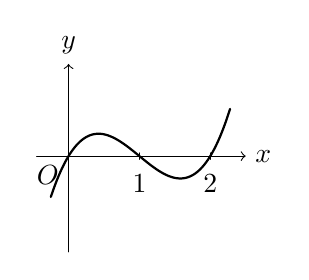
\begin{tikzpicture}[line cap=round,line join=round,scale=0.9]
  \draw[->] (-0.45,0)--(2.5,0) node[right] {$x$};
  \draw[->] (0,-1.35)--(0,1.3) node[above] {$y$};
  % A qualitative cubic crossing the x-axis at the marked 0, 1, and 2.
  \draw[thick,smooth,samples=90,domain=-0.25:2.28,variable=\t]
    plot (\t,{0.82*(\t)*(\t-1)*(\t-2)});
  \node[below left] at (0,0) {$O$};
  \draw (1,0.045)--(1,-0.045) node[below=2pt] {$1$};
  \draw (2,0.045)--(2,-0.045) node[below=2pt] {$2$};
\end{tikzpicture}
